% Chapter 5
\section{Dynamics of the String Loop} % Main chapter title

%\label{Chapter5} % For referencing the chapter elsewhere, use 

\subsection{The Dynamics of String Analysis}
The dynamics of the string loop in the lasso gripper are rooted in principles of fluid mechanics and physics \cite{abello2024string}\cite{daerr2019charmed}. This section explores the behavior of the string loop as it transitions from a low-velocity, gravity-dominated state to a high-velocity, self-supporting configuration.

At low velocities, the string loop is primarily influenced by gravity, causing it to hang downwards. This gravity-dominated regime is characterized by a noticeable sag in the string due to its light. As the velocity increases, the string undergoes a transition to a high-velocity regime where it forms a self-supporting loop. In this regime, the string is no longer suspended due to inertia but rather through the hydrodynamic drag. This drag force exerted by the surrounding air counteracts gravity, allowing the string to maintain a stable loop shape.

\begin{figure}[htbp]
\label{simulation}
\centering
\begin{tabular}{cc}
\begin{minipage}[t]{0.9\textwidth}
\centering
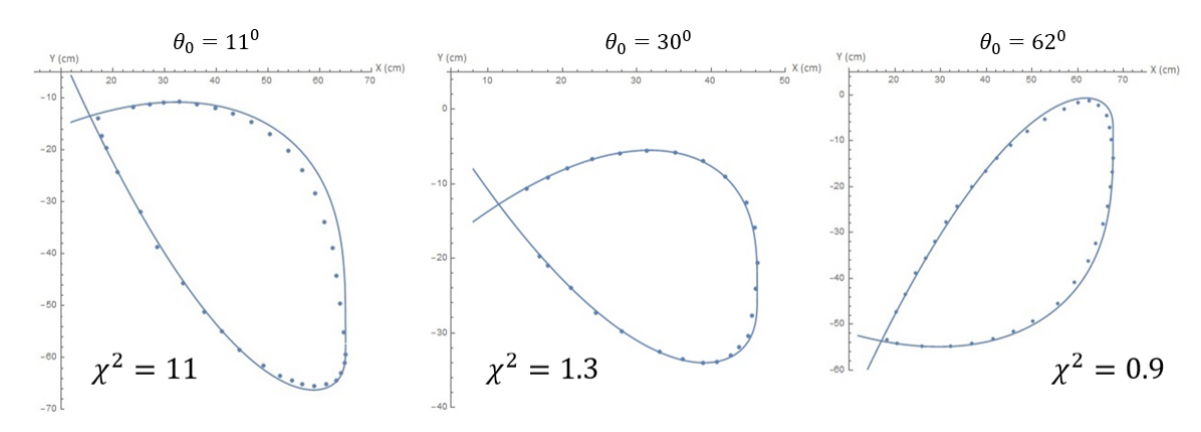
\includegraphics[width=1.0\columnwidth]{Figures/stringsim.png}
\caption{The string loop curve fitting of numerical theoretical solution with experimental profiles \cite{abello2024string}. In this case, the linear mass $\mu = 0.283 \pm 0.005 g \cdot \: m^{-1}$,  the length of the string loop $L = 160 \: cm$, shooting velocity $v = 5.1 \: m \cdot s^{-1}$ and sevel values of ejection pitch angle $\theta _0$. A satisfactory fitting result with $\chi^2 \leq 11$ is obtained.  }
\end{minipage}
\end{tabular}
\end{figure}

Assuming the loop junction is at position $s = s_0$ when $t = 0$, the position of the junction along this curve is $s = v \cdot t + s_0 (\mathrm{mod} \, L) $. $T(s)$ is noted as the tension. Frenet-Serret frame $(\vec {\tau}, \vec {n})$ is used to describe the dynamics of an infinitesimal piece of string of length $\mathrm{d}s$ subjected to its ight $\mu \mathrm{d} s \vec {g}$, its tension $\frac{\mathrm{d}(T \vec {\tau})}{\mathrm{d}s}\mathrm{d}s^3$ and the linear air drag $-f \vec {\tau} \mathrm{d} s$ where $f>0$.

Newton's motion equation produces:

\vspace{-0.3cm}
\begin{equation}
\begin{split}
\frac{\mathrm{d}(\mu v \vec {\tau})}{\mathrm{d}t} = \mu \vec {g} + \frac{\mathrm{d}(T \vec {\tau})}{\mathrm{d}s} - f \vec {\tau}
\end{split}
\end{equation}

Noting that $\mathrm{d}s = v \cdot \mathrm{d}t$, defining the effective tension $T^o = T-\mu v^2$, and recalling that $\vec {\tau} = \frac{\mathrm{d}\vec {\tau}}{\mathrm{d}s}$, the following can be obtained:

\vspace{-0.3cm}
\begin{equation}
\begin{split}
T^o \vec {\tau} - f \vec {\tau} +\mu \vec {g}s=\vec {0}
\end{split}
\end{equation}

If the origin is wisely chosen for $\vec {r}$ as the point $o$  where the tangent to the loop is vertical, the integration constants will vanish. In the vertical local FrenetSerret frame, defining $tan \theta = \frac{\mathrm{d}z}{\mathrm{d}x}$, the following can obtained:

\vspace{-0.3cm}
\begin{equation}
\begin{split}
-f \cdot ( x \mathrm{tan} \theta - z )+\mu gs=0
\end{split}
\end{equation}

This integro-differential equation can be solved analytically as figure 4.1.

The formation of the self-supporting loop is governed by the hydrodynamic drag acting on the string. Daerr et al. (2019) investigated this drag both experimentally and theoretically, focusing on a smooth long cylinder moving along its axis \cite{daerr2019charmed}. The drag force is a result of the interaction beten the moving string and the air, creating a pressure differential that lifts and supports the string loop.

The equations that characterize the shape of the string loop re formulated under the assumption of an infinitely small string radius. These equations unveil a pivotal juncture, delineating two distinct regions: a supercritical region where the wave speed along the string is less than the string's own speed, and a subcritical region where the wave speed surpasses the string's speed. This critical juncture at the interface of these regions is vital to the string loop's dynamics. Solutions to the loop equations that remain regular at this critical juncture have been derived and subsequently compared to experimental data.

In practical terms, understanding the string loop dynamics has significant implications for the lasso gripper's design and operation. By leveraging the principles of hydrodynamic drag and the transition beten different velocity regimes, the lasso gripper can achieve precise control over the string loop's shape and stability. This enables the gripper to handle objects with varying sizes and shapes effectively, ensuring a secure and reliable grip.

\section{The workspace analysis}
Due to the self-supporting loop configuration of the Lasso Gripper in three-dimensional space, the operational workspace of the proposed manipulator significantly exceeds the physical reach of the robotic arm.

\begin{figure}[ht]
    \centering
    
\includegraphics[width=0.8\linewidth]{workspace.png} 
    \caption{Lasso Gripper string loop is set at the end of UR5 robotic arm. The green point at the end of the robotic arm marks the position reachable by a rigid manipulator, while the red point indicates the furthest position on the string loop from the original point at the same robotic position.}
    \label{ws1}
\end{figure}

As delineated in Section 5.1, the three-dimensional pose kinematics of the lasso-type end-effector can be characterized by constrained dynamics under gravitational loading. For the local coordinate system constrained by gravity, the working plane is defined as the plane formed by the lasso's ejection direction and the gravity direction. The rotation with the normal vector of this working plane as the rotation axis is defined as pitch, while the rotation with the gravity vector as the rotation axis is defined as yaw. According to the right-hand coordinate system, the roll rotation axis is defined as the axis orthogonal to both the pitch and yaw rotation axes, lying within the working plane. Specifically, the gripper mechanism exhibits negligible roll angular displacement within the global coordinate frame due to gravitational stabilization. Its pitch orientation becomes parametrically dependent on the projectile's ejection velocity vector, while yaw angle variations are governed by the robotic manipulator's pose in Cartesian space.

\begin{figure}[htp]
    \centering
    
\includegraphics[width=0.6 \linewidth]{ws3.jpg} 
    \caption{The initial robotic arm workspace is marked in green and extended Lasso Gripper workspace is marked in red.}
    \label{ws2}
\end{figure}

A case study is conducted with specific parameters to investigate the working space of the Lasso Gripper on a 6-axis robotic arm using the Monte Carlo method. A UR5 robot without joint angle limitation is applied as an example in Fig. \ref{ws1}, and $[R, x_{+}, x_{-}]$ is set as $[0.7, 0.2m, 0.1m]$ in this case. The green point at the end of the robotic arm is the specific position that a rigid manipulator can reach, and the red point represents for the furthest point to the original point on the string loop at the same robotic position. The set of green points and red points in Fig. \ref{ws2} is the workspace of the robotic arm and the extended lasso gripper, respectively. Generating 200,000 sampling points for robotic arm configuration, the volume of workspace convex hull is calculated. The volume of the original UR5 workspace convex hull is $3.4620 m^3$ , and the volume of the extended Lasso Gripper workspace convex hull is $8.9002 m^3$. The workspace extending ratio is up to $157.08\%$.
